\documentclass[twocolumn, aps, floatfix]{revtex4-1}

\usepackage{graphicx}
\usepackage{fancyhdr}
\usepackage{amssymb}
\usepackage{amsmath}
\usepackage{caption}
\usepackage{enumerate}
\usepackage{subcaption}
\usepackage{textcomp}
\usepackage{placeins}
\usepackage{blindtext}

\begin{document}
\title{Lab 5. Power Matched Amplifiers and Filters }
\author{Albert Wandui}
\affiliation{EE 152: High Frequency Systems Lab.}
\maketitle

\section*{Introduction}\label{sec:introduction}
The goal of this lab is to design, assemble and test a transmission line low pass filter as well as a power matched Heterojunction Bipolar Transistor (HBT) amplifier at 4 GHz. Low pass filters have numerous applications in RF and microwave systems. A key use for low pass filters is in rejecting out of band higher order harmonics produced by non-linearities in a circuit component such as a mixer. In this lab, we designed a transmission line low pass filter with a 6 GHz cutoff. Transmission line filters made of microstrip are planar and therefore can easily be integrated into other larger components. The design of the filter is further discussed in section \ref{sec:lpdesign}.

Power amplifiers are designed primarily to maximize the power transmitted to the load. Power amplifiers are categorized based on the relative tradeoffs between maximizing power, efficiency, linearity and gain. A amplifier class designations capture the variation in the output signal within the circuit over an entire cycle of operation for a sinusoidal signal input. For this lab, we focused on class A amplifiers which are well known for their high linearity and gain and subsequently reduced efficiency and power. The efficiency of an amplifier, $\eta$ is defined as ratio of the power delivered to the load to the DC power input from the supply. A Class A amplifiers can be implemented using a single transistor in a common emitter configuration. For high gain and linearity, the transistor is biased so that it is always carrying current even when there is no signal input into the base. This DC power that is dissipated even with no signal input lowers the efficiency of the amplifier and makes it less suitable for high power applications. The gain considerations and matching networks designed for the amplifier in this lab are covered in depth in section \ref{sec:ampdesign}. 

\section*{Low Pass Filter Design}\label{sec:lpdesign}

We chose to design an odd order Butterworth filter which was first designed using lumped element components and then translated to a stepped transmission line design that was optimized for a 6 GHz cutoff. Butterworth filters have a flat response in their pass band at the cost of having a slower rolloff above cutoff frequencies. To sufficiently attenuate higher frequency signals, a higher order filter must be used. As a result, we chose to design a 5th order Butterworth to satisfy this requirement. The transfer function for the filter is usually specified for a cutoff frequency and characteristic impedance of the filter scaled to 1. With this choice of units, a 5th order Butterworth filter is fully characterized when the values $g_k, \textrm{ for } k \in \{1,2,3,4,5\}$ are fully specified. For the nth order Butterworth filter, the values are given by the relation

\begin{equation}
    g_k = 2 \sin \left[\frac{ (2 k - 1) \pi}{2 n} \right]
\end{equation}

The Butterworth filter is made of alternating series inductors and shunt capacitors. Given a normalized immitance $g_k$, the characteristic impedance $Z_0$ and the cutoff frequency $\omega_c$, we can recover the inductance and capacitance values as $L_k = g_k \frac{Z_0}{\omega_c}$ and $C_k = g_k \frac{1}{Z_0 \omega_c}$. The calculated values for inductances and capacitances have been given in table \ref{tab:parameters}.

% Change the values given in this table
\begin{table}
\centering
\begin{tabular}{l | c | c}
    \hline
    Z [$\Omega$] & W [mils] & $\lambda/4$ [mils] \\
    \hline
    50  & 44.5 & 175.0 \\
    35.36 & 73.5 & 167.5 \\
    \hline
\end{tabular}
    \caption{Parameters of the transmission lines used in the branch line coupler. All dimensions have been rounded to the nearest half mil and the values reported are the optimized values to center the circuit response at 5.9 GHz. }
    \label{tab:parameters}
\end{table}

To translate from lumped element to a stepped implementation of the filter, we noted that short sections of transmission lines with characteristic impedances $Z_{HI}$ and $Z_{LO}$ chosen such that $Z_{HI} \gg Z_0$ and $Z_{LO} \ll Z_0$ can be used as inductors and capacitors respectively. We chose the impedances of the transmission lines by choosing the width of the microstrip line. For $Z_{HI} = 97.57 \Omega$, we used 6 mil wide microstrip, while for $Z_{LO} = 29.73 \Omega$, we used 120 mil wide microstrip lines. With the choice of impedance fixed, the value of the inductance or capacitance is determined by the electrical length $\beta l$ of the microstrip section. For the inductive case, $\beta l = g_k \frac{Z_0}{Z_{HI}}$ and for the capacitive case $\beta l = g_k \frac{Z_{LO}}{Z_0} $. Using the TX Line tool in MWO, we were able to calculate the physical length of the microstrip lines once the electrical length was specified using the equations given. These values have also been given in table \ref{tab:parameters}. 

% \ref{fig:steppedschematic}

A circuit schematic was assembled in MWO as shown in figure FIX THIS . To better model the physical circuit, we used the microstrip MSTEP elements, based on electromagnetic (EM) simulations, to capture the discontinuity in line width in moving from high impedance to low impedance sections of the filters. The circuit was simulated and we optimized the circuit to achieve cutoff at exactly 6 GHz. Since odd order Butterworth filters are symmetric about their midplane, we tune only 3 line lengths for the 5 element filters. Figure \ref{fig:lumpedvsstepped} shows a comparison of the simulation results between a stepped and a lumped element fifth order filter. Both filters show very similar responses in their passband and with similar cutoffs. However, the roll-off for the stepped implementation is much shallower than the lumped element case. This is because the stepped filter does not attenuate signals at arbitrarily high frequencies. Infact, the filter response repeats as a series of passbands and attenuated bands as you move to higher frequencies. 

%Need to include figures for the lumped element and stepped filter circuit schematics.

\begin{figure}
    \centering
    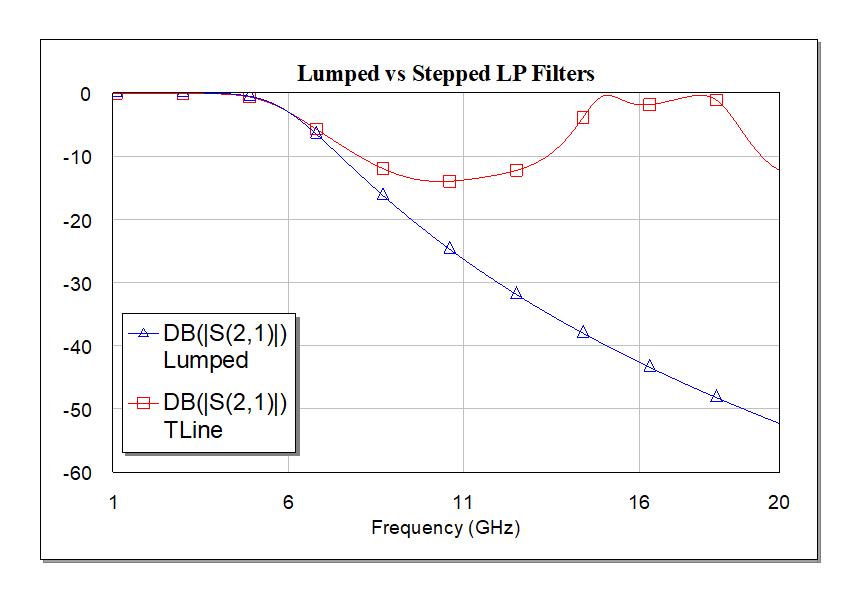
\includegraphics[scale=0.4]{lumped_vs_stepped.png}
    \caption{A comparison between the lumped and stepped implementation of the Butterworth filters. The stepped implementation has a higher passband starting at about 14 GHz.}
    \label{fig:lumpedvsstepped}
\end{figure}

\section*{Amplifier Design}\label{sec:ampdesign}
The goal of the amplifier design was to maximize the transducer gain, $G_T$ of the amplifier. The transducer gain is defined as the ratio of the power delivered to the load to the available power from the source. The power delivered to the load with a reflection coefficient, $\Gamma_l$ by the two port network of the amplifier is given by $P_{del} = |b_2|^2 \left(1 - |\Gamma_l|^2\right) $. The power available from the source with source power $|a_s|^2$ and a reflection coefficient $\Gamma_s$ is given by $P_{avs} = |a_s|^2 /\left(1 - |\Gamma_s|^2 \right)$. Combining these two expressions and using Mason's rule to find $b_2$, we can reexpress the transducer gain as 

\begin{equation}
    G_T = \frac{1 - |\Gamma_s|^2}{|1 - \Gamma_s \Gamma_{in}|^2} \times |S_{21}|^2 \times \frac{1  - |\Gamma_l|^2}{|1 - \Gamma_l S_{22}|^2}
    \label{eqn:transducergain}
\end{equation}

Here, $\Gamma_{in} = S_{11} + \frac{S_{21} \Gamma_l S_{12}}{1 - S_{22} \Gamma_l}$ is the input impedance of the amplifier with the load connected to it. From equation \ref{eqn:transducergain}, we can conclude that in order to maximize the gain, two conditions must be satisfied; $\Gamma_s = \Gamma_{in}^*$ and $\Gamma_l = S_{22}^*$ in addition to making $|S_{21}|$ as large as possible. The value of $S_{21}$ is a function of the biasing conditions of the amplifier. As a result, we maximized it by choosing the transistor bias of 2 V with 20 mA current at the output of the transistor network. The biasing circuit used for the transistor is shown in figure \ref{fig:ampbiasschematic}. 

\begin{figure*}
    \centering
    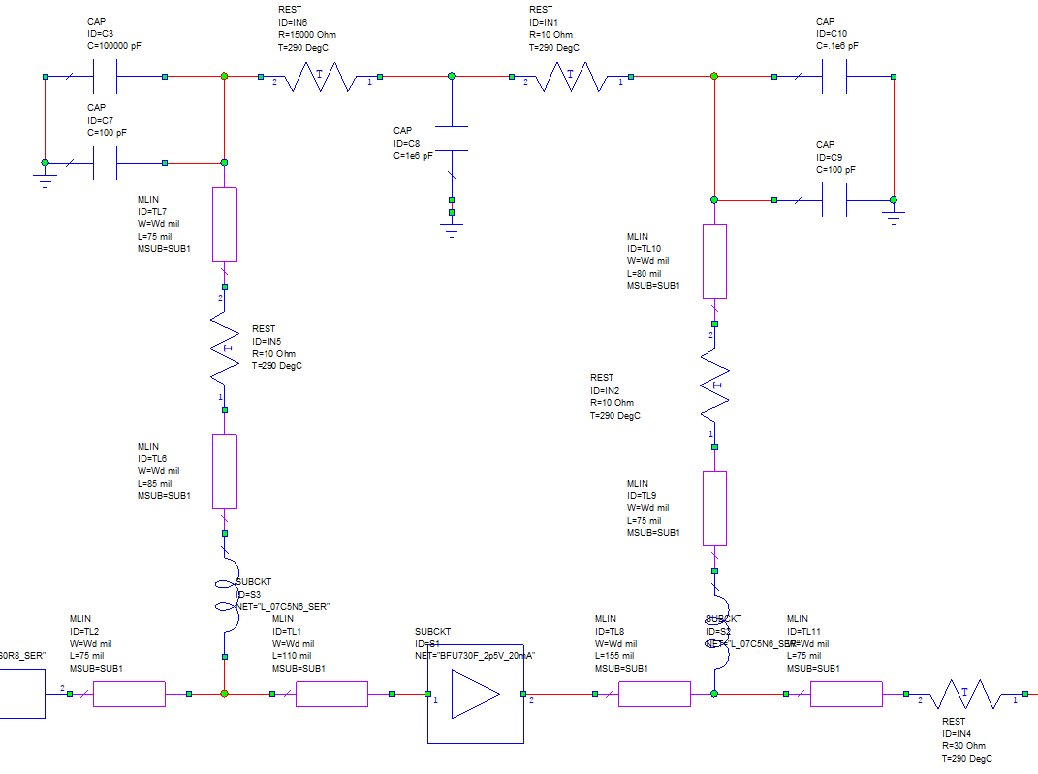
\includegraphics[scale=0.6]{Biasing_Network.png}
    \caption{The biasing network chosen to achieve 2 V at the output with 20 mA collector current. The inductors in the biasing network are used for amplifier stability.}
    \label{fig:ampbiasschematic}
\end{figure*}

With the bias chosen, we then designed a matching network at the transistor output to transform the $50 \Omega$ load to one that satisfies $\Gamma_l = S_{22}^*$. We designed the matching network using lumped element capacitors and inductors. For the output matching, a single 1 nH inductor sufficed to give a FIX THIS match at 6 GHz. The output matching network is shown in figure \ref{fig:outputmatch} and the level of match achieved is shown in figure FIX THIS.


\begin{figure}
    \centering
    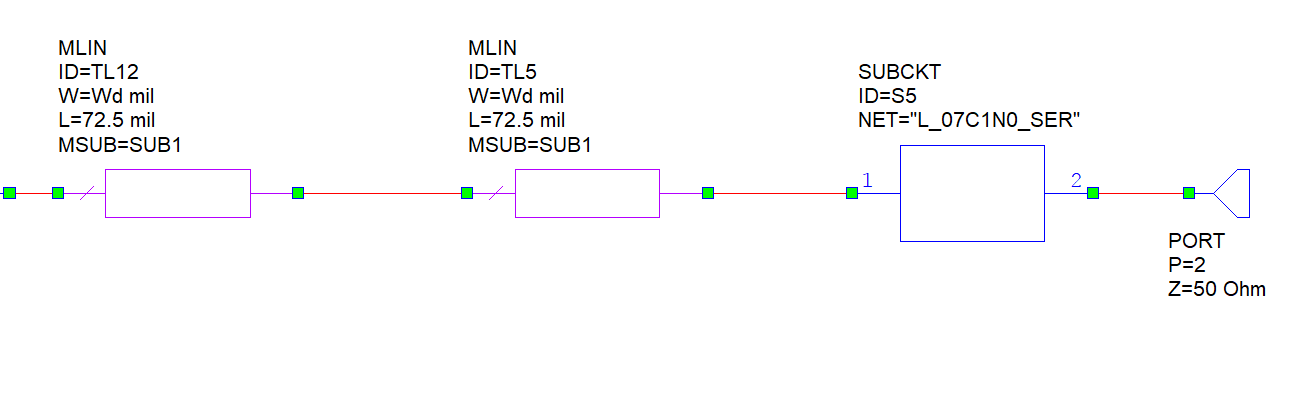
\includegraphics[scale=0.4]{output_matching_network.png}
    \caption{Output matching network for the power amplifier.}
    \label{fig:outputmatch}
\end{figure}


The output matching network fixes $\Gamma_l$ which sets the value of $\Gamma_{in}$ for the input matching network. We again designed the input matching network using a combination of series capacitors and shunt inductors as shown in figure \ref{fig:inputmatch}. 

\begin{figure}
    \centering
    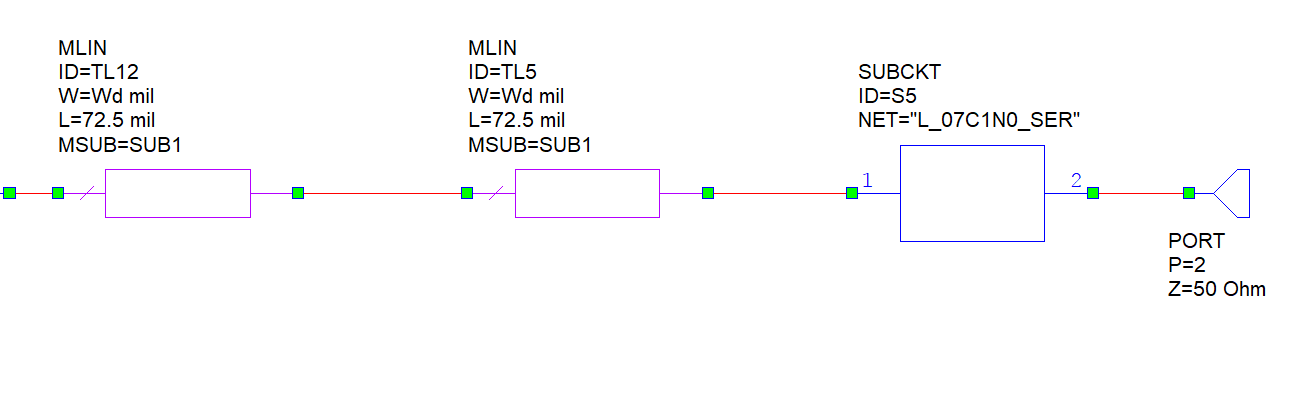
\includegraphics[scale=0.4]{output_matching_network.png}
    \caption{Output matching network for the power amplifier.}
    \label{fig:inputmatch}
\end{figure}

With the choice of input and output matching networks, we expected to achieve a transducer gain of 16 dB at 6 GHz as shown in figure FIX THIS.

\section*{Lab Testing}\label{sec:testing}


\section*{Analysis}\label{sec:analysis}


\section*{Conclusions}

\end{document}